\documentclass[twoside]{book}

% Packages required by doxygen
\usepackage{fixltx2e}
\usepackage{calc}
\usepackage{doxygen}
\usepackage[export]{adjustbox} % also loads graphicx
\usepackage{graphicx}
\usepackage[utf8]{inputenc}
\usepackage{makeidx}
\usepackage{multicol}
\usepackage{multirow}
\PassOptionsToPackage{warn}{textcomp}
\usepackage{textcomp}
\usepackage[nointegrals]{wasysym}
\usepackage[table]{xcolor}

% Font selection
\usepackage[T1]{fontenc}
\usepackage[scaled=.90]{helvet}
\usepackage{courier}
\usepackage{amssymb}
\usepackage{sectsty}
\renewcommand{\familydefault}{\sfdefault}
\allsectionsfont{%
  \fontseries{bc}\selectfont%
  \color{darkgray}%
}
\renewcommand{\DoxyLabelFont}{%
  \fontseries{bc}\selectfont%
  \color{darkgray}%
}
\newcommand{\+}{\discretionary{\mbox{\scriptsize$\hookleftarrow$}}{}{}}

% Page & text layout
\usepackage{geometry}
\geometry{%
  a4paper,%
  top=2.5cm,%
  bottom=2.5cm,%
  left=2.5cm,%
  right=2.5cm%
}
\tolerance=750
\hfuzz=15pt
\hbadness=750
\setlength{\emergencystretch}{15pt}
\setlength{\parindent}{0cm}
\setlength{\parskip}{3ex plus 2ex minus 2ex}
\makeatletter
\renewcommand{\paragraph}{%
  \@startsection{paragraph}{4}{0ex}{-1.0ex}{1.0ex}{%
    \normalfont\normalsize\bfseries\SS@parafont%
  }%
}
\renewcommand{\subparagraph}{%
  \@startsection{subparagraph}{5}{0ex}{-1.0ex}{1.0ex}{%
    \normalfont\normalsize\bfseries\SS@subparafont%
  }%
}
\makeatother

% Headers & footers
\usepackage{fancyhdr}
\pagestyle{fancyplain}
\fancyhead[LE]{\fancyplain{}{\bfseries\thepage}}
\fancyhead[CE]{\fancyplain{}{}}
\fancyhead[RE]{\fancyplain{}{\bfseries\leftmark}}
\fancyhead[LO]{\fancyplain{}{\bfseries\rightmark}}
\fancyhead[CO]{\fancyplain{}{}}
\fancyhead[RO]{\fancyplain{}{\bfseries\thepage}}
\fancyfoot[LE]{\fancyplain{}{}}
\fancyfoot[CE]{\fancyplain{}{}}
\fancyfoot[RE]{\fancyplain{}{\bfseries\scriptsize Generated by Doxygen }}
\fancyfoot[LO]{\fancyplain{}{\bfseries\scriptsize Generated by Doxygen }}
\fancyfoot[CO]{\fancyplain{}{}}
\fancyfoot[RO]{\fancyplain{}{}}
\renewcommand{\footrulewidth}{0.4pt}
\renewcommand{\chaptermark}[1]{%
  \markboth{#1}{}%
}
\renewcommand{\sectionmark}[1]{%
  \markright{\thesection\ #1}%
}

% Indices & bibliography
\usepackage{natbib}
\usepackage[titles]{tocloft}
\setcounter{tocdepth}{3}
\setcounter{secnumdepth}{5}
\makeindex

% Hyperlinks (required, but should be loaded last)
\usepackage{ifpdf}
\ifpdf
  \usepackage[pdftex,pagebackref=true]{hyperref}
\else
  \usepackage[ps2pdf,pagebackref=true]{hyperref}
\fi
\hypersetup{%
  colorlinks=true,%
  linkcolor=blue,%
  citecolor=blue,%
  unicode%
}

% Custom commands
\newcommand{\clearemptydoublepage}{%
  \newpage{\pagestyle{empty}\cleardoublepage}%
}

\usepackage{caption}
\captionsetup{labelsep=space,justification=centering,font={bf},singlelinecheck=off,skip=4pt,position=top}

%===== C O N T E N T S =====

\begin{document}

% Titlepage & ToC
\hypersetup{pageanchor=false,
             bookmarksnumbered=true,
             pdfencoding=unicode
            }
\pagenumbering{roman}
\begin{titlepage}
\vspace*{7cm}
\begin{center}%
{\Large Simple I\+EC 61850 Client }\\
\vspace*{1cm}
{\large Generated by Doxygen 1.8.11}\\
\end{center}
\end{titlepage}
\clearemptydoublepage
\tableofcontents
\clearemptydoublepage
\pagenumbering{arabic}
\hypersetup{pageanchor=true}

%--- Begin generated contents ---
\chapter{File Index}
\section{File List}
Here is a list of all documented files with brief descriptions\+:\begin{DoxyCompactList}
\item\contentsline{section}{src/\hyperlink{simple-iec61850-client_8c}{simple-\/iec61850-\/client.\+c} \\*Test Class }{\pageref{simple-iec61850-client_8c}}{}
\end{DoxyCompactList}

\chapter{File Documentation}
\hypertarget{simple-iec61850-client_8c}{}\section{src/simple-\/iec61850-\/client.c File Reference}
\label{simple-iec61850-client_8c}\index{src/simple-\/iec61850-\/client.\+c@{src/simple-\/iec61850-\/client.\+c}}


Test Class.  


{\ttfamily \#include \char`\"{}iec61850\+\_\+client.\+h\char`\"{}}\\*
{\ttfamily \#include \char`\"{}hal\+\_\+thread.\+h\char`\"{}}\\*
{\ttfamily \#include $<$stdlib.\+h$>$}\\*
{\ttfamily \#include $<$stdio.\+h$>$}\\*
{\ttfamily \#include \char`\"{}argp.\+h\char`\"{}}\\*
{\ttfamily \#include $<$unistd.\+h$>$}\\*
Include dependency graph for simple-\/iec61850-\/client.c\+:\nopagebreak
\begin{figure}[H]
\begin{center}
\leavevmode
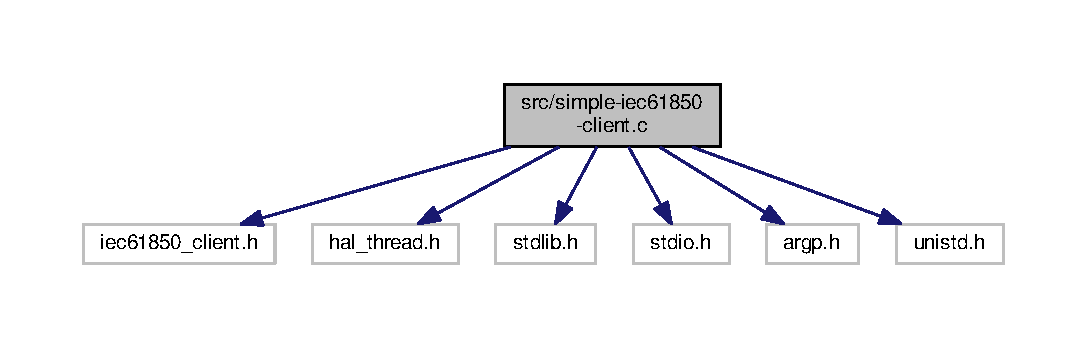
\includegraphics[width=350pt]{simple-iec61850-client_8c__incl}
\end{center}
\end{figure}
\subsection*{Functions}
\begin{DoxyCompactItemize}
\item 
void \hyperlink{simple-iec61850-client_8c_a19c4ac63742805a0bfd8fc4a512b42d3}{run\+Client} ()
\begin{DoxyCompactList}\small\item\em Function which starts the client and checks the status. \end{DoxyCompactList}\item 
static int \hyperlink{simple-iec61850-client_8c_aaf7bc24f3891f0c63a6043f4dc2ab311}{parse\+\_\+opt} (int key, char $\ast$arg, struct argp\+\_\+state $\ast$state)
\begin{DoxyCompactList}\small\item\em Function which parses the given options and arguments. \end{DoxyCompactList}\item 
int \hyperlink{simple-iec61850-client_8c_a3c04138a5bfe5d72780bb7e82a18e627}{main} (int argc, char $\ast$$\ast$argv)
\begin{DoxyCompactList}\small\item\em Main function. \end{DoxyCompactList}\end{DoxyCompactItemize}
\subsection*{Variables}
\begin{DoxyCompactItemize}
\item 
char $\ast$ \hyperlink{simple-iec61850-client_8c_a1c2046dcb30a629d6d9f45ff8f403f12}{host}
\begin{DoxyCompactList}\small\item\em Global variable for the hostname. \end{DoxyCompactList}\item 
int \hyperlink{simple-iec61850-client_8c_ac31354d08316076b496efb2b3a2c69e6}{tcp\+Port} = 10102
\begin{DoxyCompactList}\small\item\em Global variable for the T\+CP Port. \end{DoxyCompactList}\item 
int \hyperlink{simple-iec61850-client_8c_ad43c3812e6d13e0518d9f8b8f463ffcf}{count} = -\/1
\begin{DoxyCompactList}\small\item\em Global variable for number of requests. \end{DoxyCompactList}\item 
int \hyperlink{simple-iec61850-client_8c_a7c0b25939579bd308b11966fb04288e0}{sleep\+Int} = 1
\begin{DoxyCompactList}\small\item\em Global variable for the time between sending requests. \end{DoxyCompactList}\end{DoxyCompactItemize}


\subsection{Detailed Description}
Test Class. 

More Details to Test Class

\begin{DoxyAuthor}{Author}
David Mittelstädt 
\end{DoxyAuthor}
\begin{DoxySeeAlso}{See also}
\href{https://github.com/dmittelstaedt/siprenz-protocols}{\tt https\+://github.\+com/dmittelstaedt/siprenz-\/protocols} 

\href{http://libiec61850.com/libiec61850/}{\tt http\+://libiec61850.\+com/libiec61850/} 
\end{DoxySeeAlso}


\subsection{Function Documentation}
\index{simple-\/iec61850-\/client.\+c@{simple-\/iec61850-\/client.\+c}!main@{main}}
\index{main@{main}!simple-\/iec61850-\/client.\+c@{simple-\/iec61850-\/client.\+c}}
\subsubsection[{\texorpdfstring{main(int argc, char $\ast$$\ast$argv)}{main(int argc, char **argv)}}]{\setlength{\rightskip}{0pt plus 5cm}int main (
\begin{DoxyParamCaption}
\item[{int}]{argc, }
\item[{char $\ast$$\ast$}]{argv}
\end{DoxyParamCaption}
)}\hypertarget{simple-iec61850-client_8c_a3c04138a5bfe5d72780bb7e82a18e627}{}\label{simple-iec61850-client_8c_a3c04138a5bfe5d72780bb7e82a18e627}


Main function. 

Details of the function. 
\begin{DoxyParams}{Parameters}
{\em argc} & Number of arguments \\
\hline
{\em argv} & Content of the arguments \\
\hline
\end{DoxyParams}
\begin{DoxyReturn}{Returns}
Exit status of the application 
\end{DoxyReturn}
\index{simple-\/iec61850-\/client.\+c@{simple-\/iec61850-\/client.\+c}!parse\+\_\+opt@{parse\+\_\+opt}}
\index{parse\+\_\+opt@{parse\+\_\+opt}!simple-\/iec61850-\/client.\+c@{simple-\/iec61850-\/client.\+c}}
\subsubsection[{\texorpdfstring{parse\+\_\+opt(int key, char $\ast$arg, struct argp\+\_\+state $\ast$state)}{parse_opt(int key, char *arg, struct argp_state *state)}}]{\setlength{\rightskip}{0pt plus 5cm}static int parse\+\_\+opt (
\begin{DoxyParamCaption}
\item[{int}]{key, }
\item[{char $\ast$}]{arg, }
\item[{struct argp\+\_\+state $\ast$}]{state}
\end{DoxyParamCaption}
)\hspace{0.3cm}{\ttfamily [static]}}\hypertarget{simple-iec61850-client_8c_aaf7bc24f3891f0c63a6043f4dc2ab311}{}\label{simple-iec61850-client_8c_aaf7bc24f3891f0c63a6043f4dc2ab311}


Function which parses the given options and arguments. 

Details of the function. 
\begin{DoxyParams}{Parameters}
{\em Key} & \\
\hline
{\em Value} & of argument \\
\hline
{\em Struct} & \\
\hline
\end{DoxyParams}
\begin{DoxyReturn}{Returns}
Return code of parsing the arguments 
\end{DoxyReturn}
\index{simple-\/iec61850-\/client.\+c@{simple-\/iec61850-\/client.\+c}!run\+Client@{run\+Client}}
\index{run\+Client@{run\+Client}!simple-\/iec61850-\/client.\+c@{simple-\/iec61850-\/client.\+c}}
\subsubsection[{\texorpdfstring{run\+Client()}{runClient()}}]{\setlength{\rightskip}{0pt plus 5cm}void run\+Client (
\begin{DoxyParamCaption}
{}
\end{DoxyParamCaption}
)}\hypertarget{simple-iec61850-client_8c_a19c4ac63742805a0bfd8fc4a512b42d3}{}\label{simple-iec61850-client_8c_a19c4ac63742805a0bfd8fc4a512b42d3}


Function which starts the client and checks the status. 

Details of the function. 

\subsection{Variable Documentation}
\index{simple-\/iec61850-\/client.\+c@{simple-\/iec61850-\/client.\+c}!count@{count}}
\index{count@{count}!simple-\/iec61850-\/client.\+c@{simple-\/iec61850-\/client.\+c}}
\subsubsection[{\texorpdfstring{count}{count}}]{\setlength{\rightskip}{0pt plus 5cm}int count = -\/1}\hypertarget{simple-iec61850-client_8c_ad43c3812e6d13e0518d9f8b8f463ffcf}{}\label{simple-iec61850-client_8c_ad43c3812e6d13e0518d9f8b8f463ffcf}


Global variable for number of requests. 

Details. \index{simple-\/iec61850-\/client.\+c@{simple-\/iec61850-\/client.\+c}!host@{host}}
\index{host@{host}!simple-\/iec61850-\/client.\+c@{simple-\/iec61850-\/client.\+c}}
\subsubsection[{\texorpdfstring{host}{host}}]{\setlength{\rightskip}{0pt plus 5cm}char$\ast$ host}\hypertarget{simple-iec61850-client_8c_a1c2046dcb30a629d6d9f45ff8f403f12}{}\label{simple-iec61850-client_8c_a1c2046dcb30a629d6d9f45ff8f403f12}


Global variable for the hostname. 

Details. \index{simple-\/iec61850-\/client.\+c@{simple-\/iec61850-\/client.\+c}!sleep\+Int@{sleep\+Int}}
\index{sleep\+Int@{sleep\+Int}!simple-\/iec61850-\/client.\+c@{simple-\/iec61850-\/client.\+c}}
\subsubsection[{\texorpdfstring{sleep\+Int}{sleepInt}}]{\setlength{\rightskip}{0pt plus 5cm}int sleep\+Int = 1}\hypertarget{simple-iec61850-client_8c_a7c0b25939579bd308b11966fb04288e0}{}\label{simple-iec61850-client_8c_a7c0b25939579bd308b11966fb04288e0}


Global variable for the time between sending requests. 

Details. \index{simple-\/iec61850-\/client.\+c@{simple-\/iec61850-\/client.\+c}!tcp\+Port@{tcp\+Port}}
\index{tcp\+Port@{tcp\+Port}!simple-\/iec61850-\/client.\+c@{simple-\/iec61850-\/client.\+c}}
\subsubsection[{\texorpdfstring{tcp\+Port}{tcpPort}}]{\setlength{\rightskip}{0pt plus 5cm}int tcp\+Port = 10102}\hypertarget{simple-iec61850-client_8c_ac31354d08316076b496efb2b3a2c69e6}{}\label{simple-iec61850-client_8c_ac31354d08316076b496efb2b3a2c69e6}


Global variable for the T\+CP Port. 

Details. 
%--- End generated contents ---

% Index
\backmatter
\newpage
\phantomsection
\clearemptydoublepage
\addcontentsline{toc}{chapter}{Index}
\printindex

\end{document}
